\section{Experiments using Error Confinement for JPEG} \label{sec:exp}
To combine with proposed error confinement technique, we adopt simple parity bit as the error detection mechanism, which incurs 1 bit overhead for encoding 32 bits data. In this section, we benchmark the proposed approach with SECDED under Hamming code scheme $H[38, 32]$.

The proposed technique is tested in the processor architecture from Section \ref{sec:qos_asip}. Figure \ref{fig:qos_program} shows an code snapshot of the programming example with introduced custom instructions for DCT. The generalized $8 \times 8$ matrices are stored as reference Look-up-Table. DCT and quantization data are encoded using parity bits during store access. Each read access to the DCT and quantization coefficient checks its correctness using previously encoded parity encoding. In case of a detected error, reference value replace the wrong value directly. The quality of output image is evaluated using the PSNR.

\begin{figure}
\centering
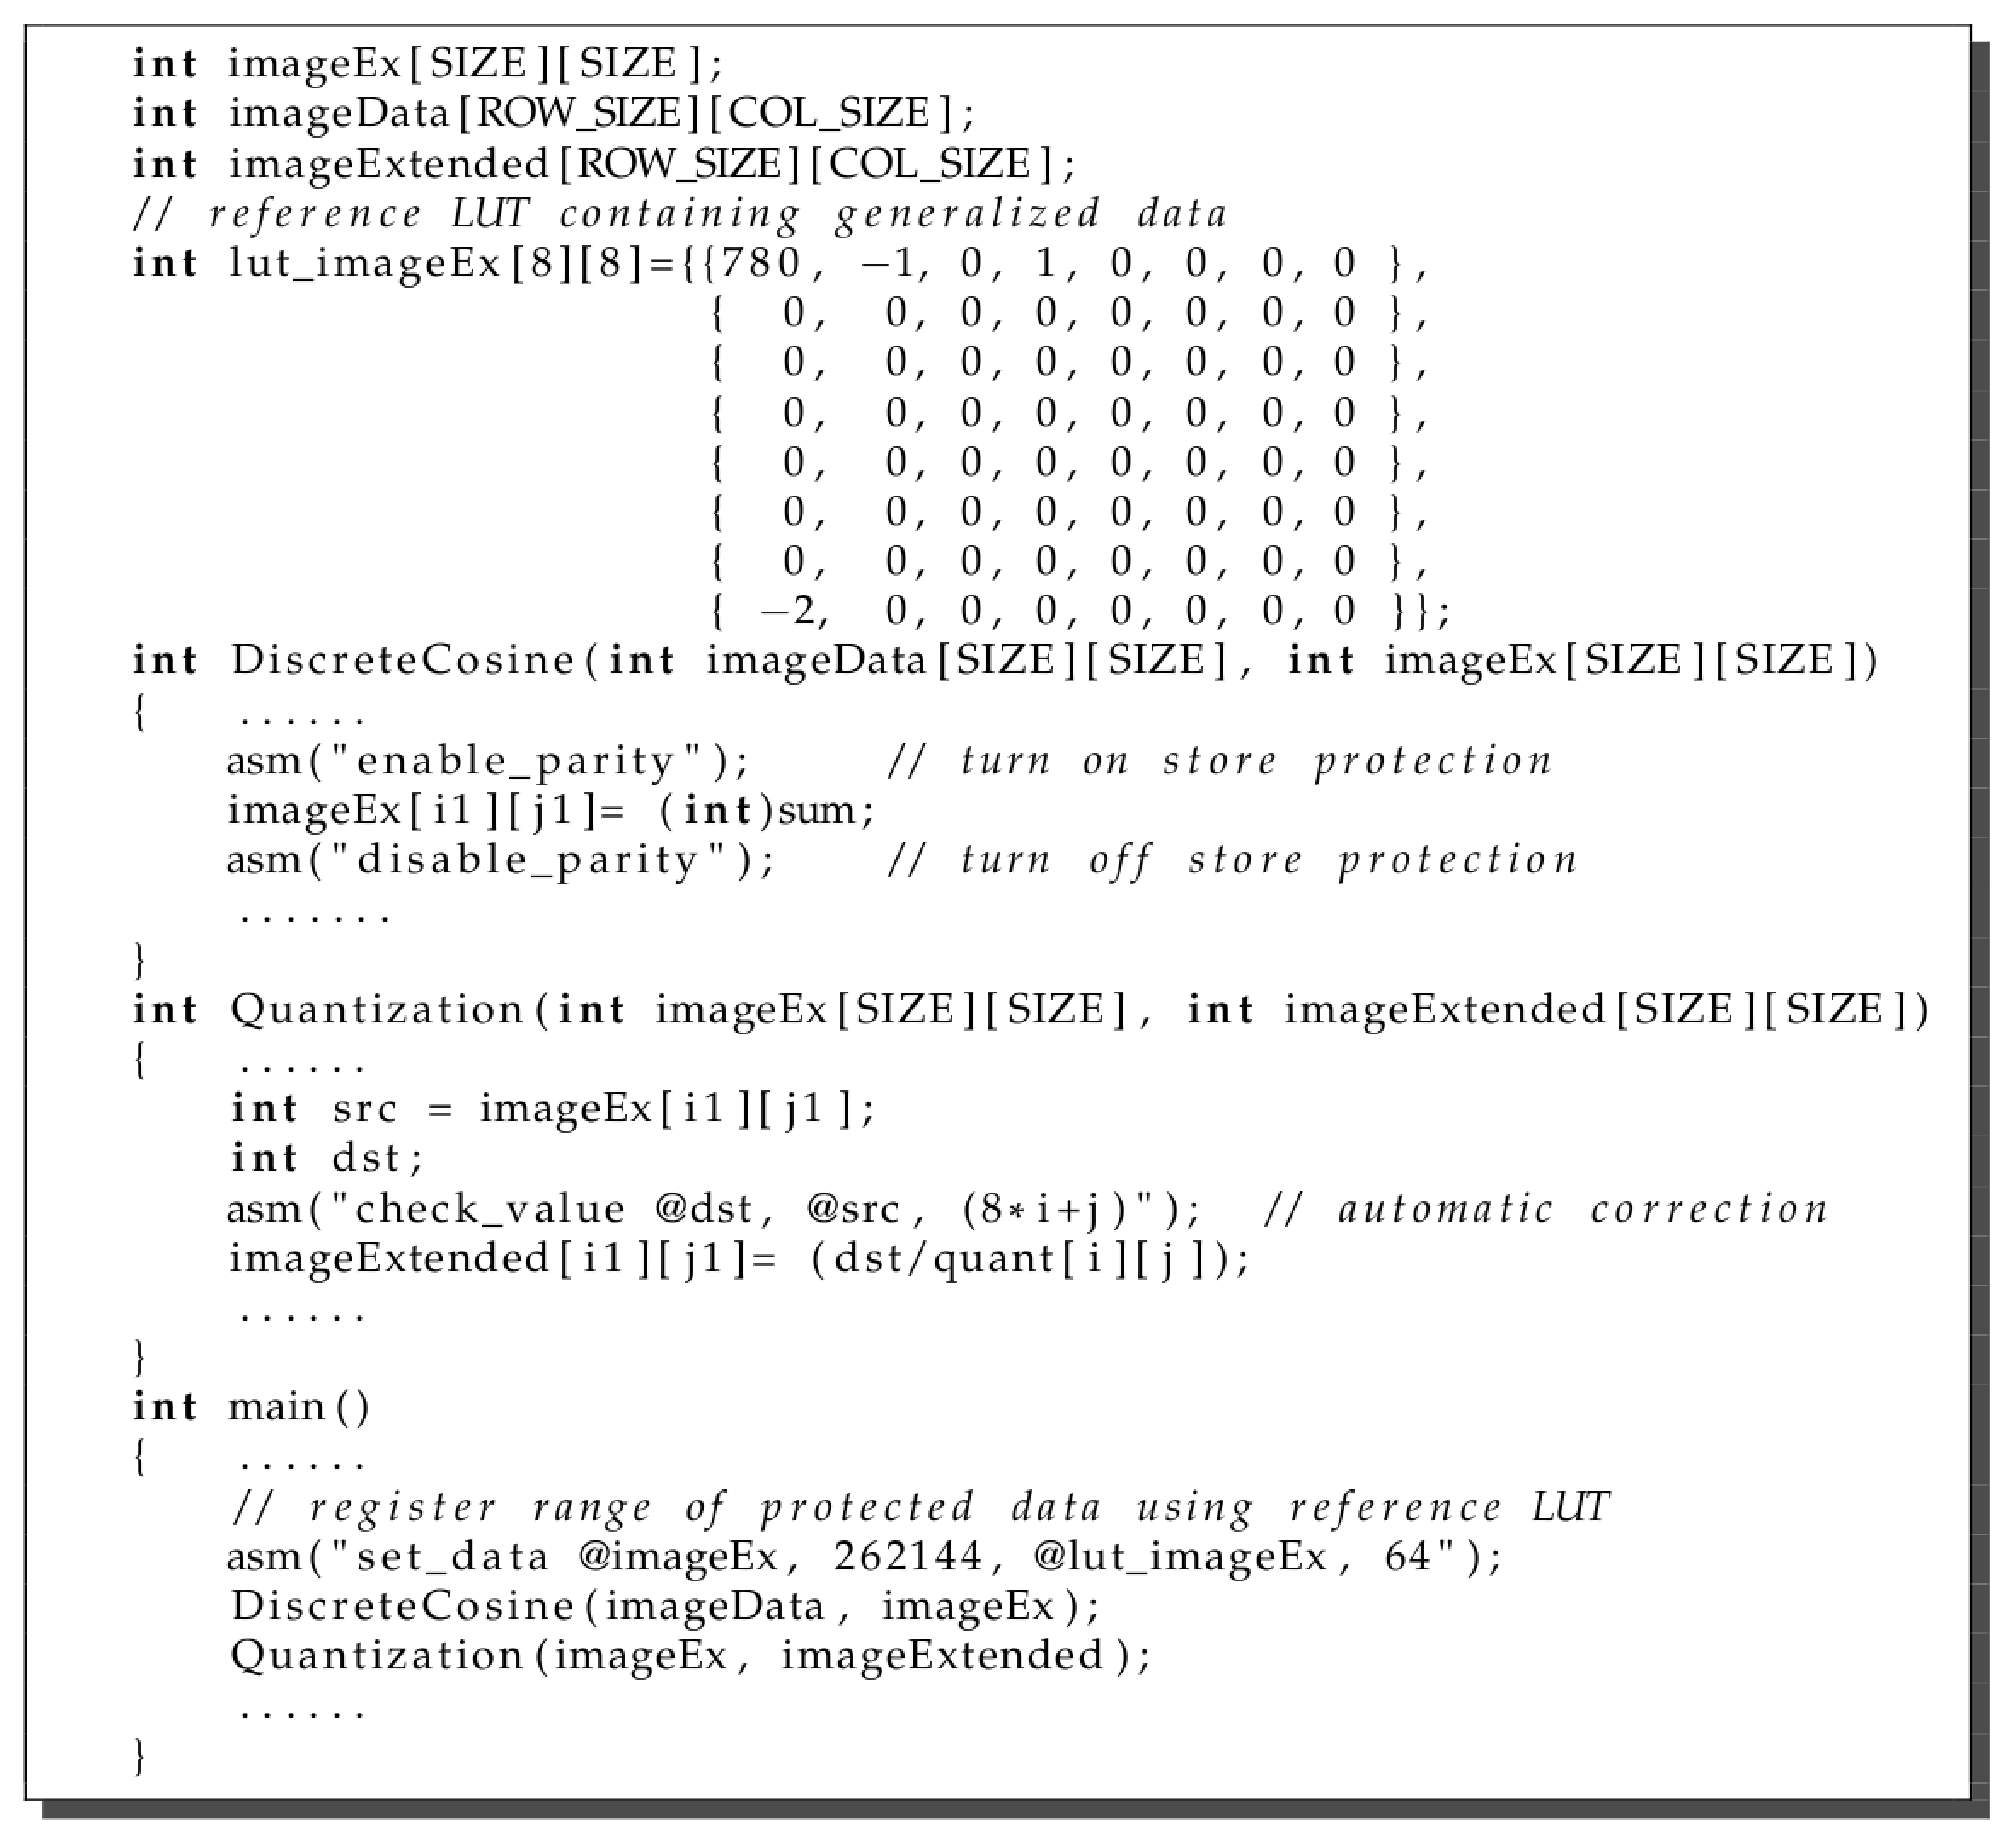
\includegraphics[width=80mm]{./eps/qos_program}
\caption{Programming example with custom instructions for DCT}
\vspace{-4mm}
\label{fig:qos_program}
\end{figure}

% \lstinputlisting[basicstyle=\tiny,  float=h, language=C, label=list:qos_program, caption=Programming example with custom instructions for DCT, captionpos=b]{./eps/approximate_dct.c}

\subsection{PSNR under Error Injection}

First the single bit errors are randomly injected to the memory location of $512 \times 512$ words and parity bits storing the DCT output coefficients, which are protected using the proposed approach. Figure \ref{fig:qos_lena}(c-f) shows the JPEG output images and corresponding PSNR values with different amounts of single bitflips under proposed protection scheme. The result shows that under 800 bitfilps, the PSNR of the image is still of 36.24 dB, which is 7.6\% of degradation with regard to the  free output. A scheme with 1,000 bitflips will reduce the PSNR of image to 23.68 dB, which is hardly acceptable. The reason for such strong degradation is that the first 20 DCT coefficient of the $8 \times 8$ matrix, which occurs 85\% of the input image quality, are injected with two bitflips in the same data word under 1,000 bitflips, so that the parity is not able to detect such schemes. In contrast, Figure  \ref{fig:qos_lena}(a, b) show the output image without protection. Even one single bitflip gives an output PSNR of -0.03 dB.

\begin{figure}
\centering
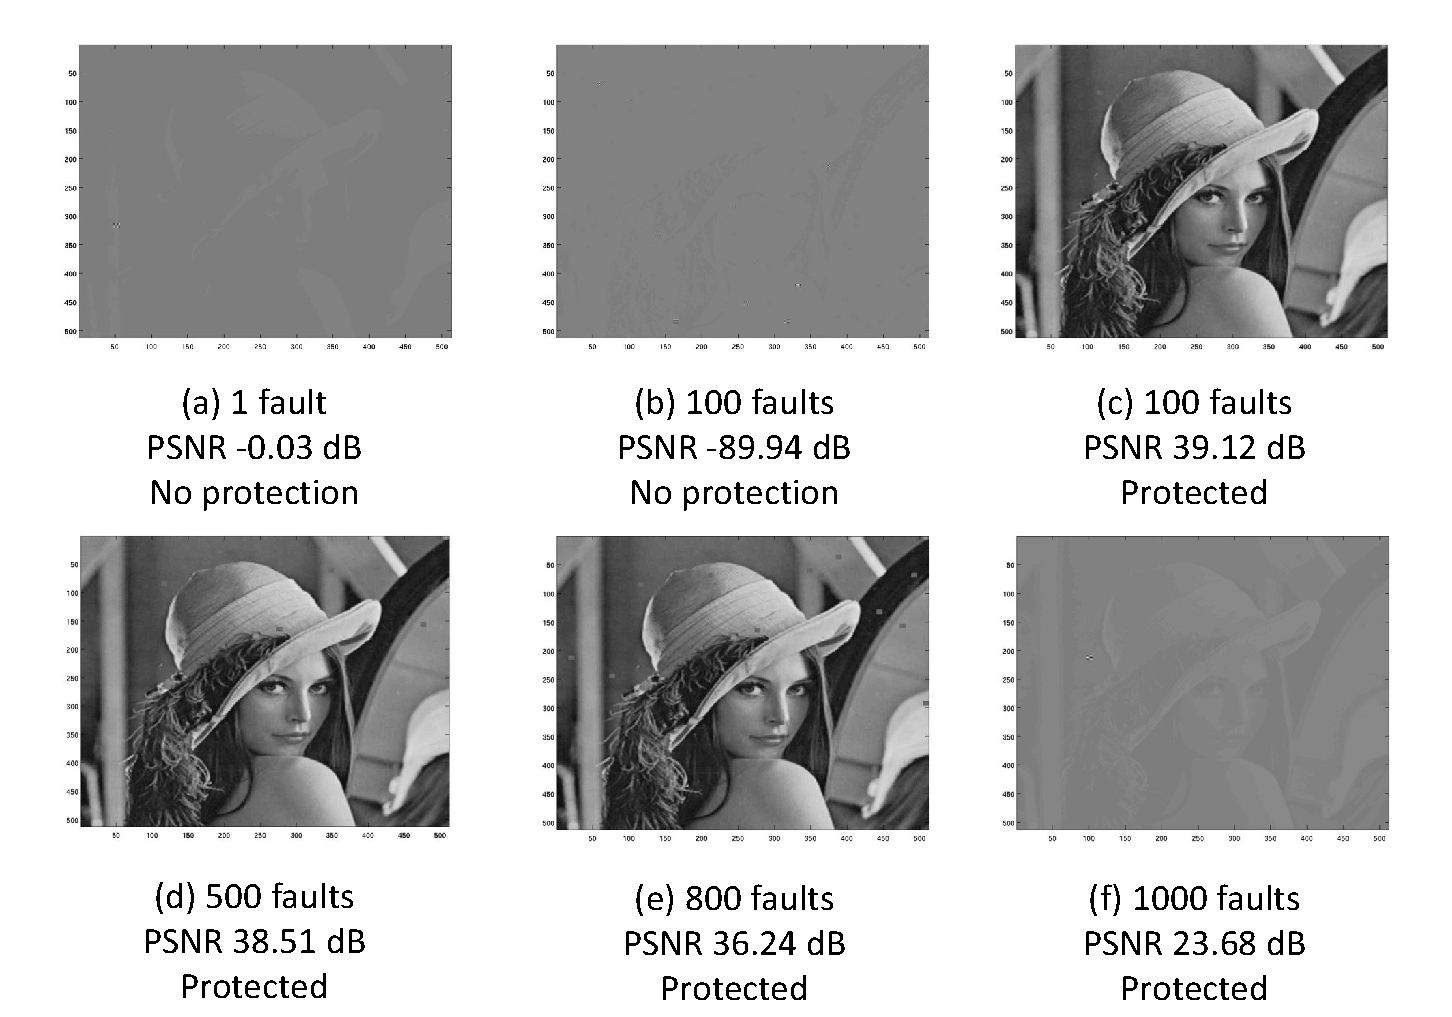
\includegraphics[width=90mm]{./eps/qos_lena}
\caption{Output images under different schemes of error injection}
\vspace{-4mm}
\label{fig:qos_lena}
\end{figure}

We benchmark the proposed protection with ECC and present the PSNR trends with the amount of single bitflips in Figure \ref{fig:qos_snr}. Results for protection of DCT and quantization coefficients are presented in Figure \ref{fig:qos_snr}a) and b) respectively. As number of single bitflips increases, the output quality using error confinement reduces slightly faster compared with ECC scheme. This results from the fact that the proposed approach substitutes the wrong data with the averaged value from pre-evaluation, which is inaccurate to some extent. However, ECC corrects all single bit errors. Note that the inaccurate correction caused by the proposed approach still gives the output image with PSNR above 36 dB under 800 errors, which closely approximates the error free image. For 900 errors both methods fail to produce a qualified image. We reason the failure of this and find out that for ECC, the intrinsic SECDED hamming code fails to correct the error of two bitflips. On the contrary, the proposed approach fails because the low cost parity bit can not detect two bitflips per data word.

Compared between different protected data, quantization coefficients are more vulnerable than the DCT coefficients. The PSNR is only 1.37 dB using proposed approach and 1.22 dB using ECC for 900 single bitflips. The reason is that the quantization coefficients are sparse in the sense that most of them are zero. The uncorrectable errors on the rest nonzero coefficients disturb the image quality more significantly than the dense DCT coefficients.

\begin{figure}
\centering
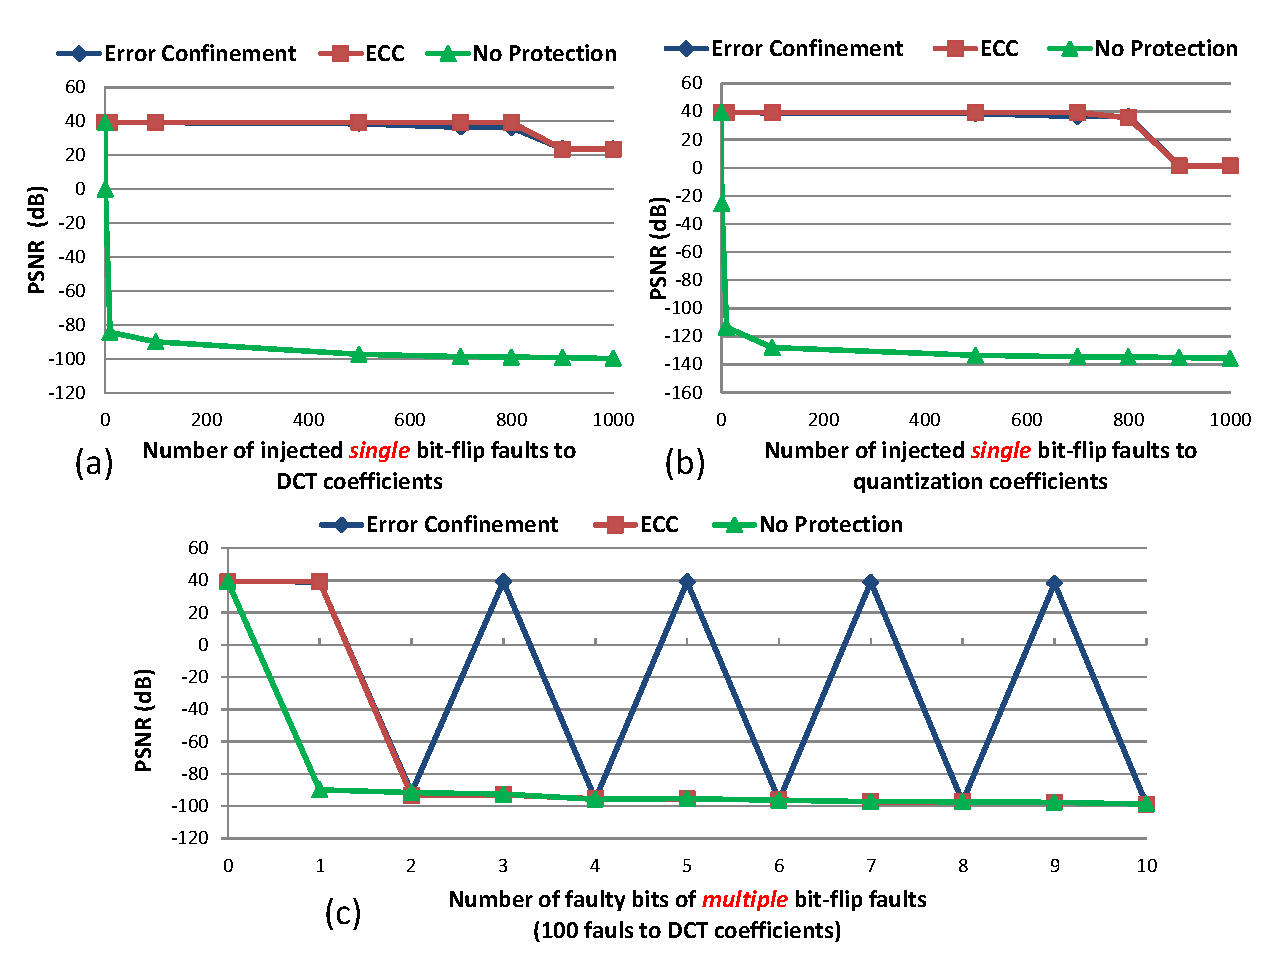
\includegraphics[width=90mm]{./eps/qos_snr}
\caption{PSNR under no protection, error confinement protection and ECC protection schemes}
\vspace{-4mm}
\label{fig:qos_snr}
\end{figure}

Error confinement enables the possibility to correct multiple bitflip error in single data word, which prevents the output image from the unrecoverable damage. We test such advantage using multiple bits injection and benchmark with ECC. Figure \ref{fig:qos_snr}c) shows the trendline between the amount of bitflips in single data word and the output image PSNR. A total number of 100 multi-bitflip errors are injected to the DCT coefficients. It is observed that the resulted PSNR of the proposed approach is above 38 dB for all errors with odd number of erroneous bits per data word, which are detectable by simple parity bit. For those with even number of erroneous bits, the output image quality is unacceptable since parity bit itself fails error detection. In contrast, ECC protection gives constantly low PSNR values regardless of number of erroneous bits per data word, since it cannot correct more than one bit error. This indicates that the proposed approach can achieve even better protection combined with more efficient error detection techniques.

The subfigures in Figure \ref{fig:qos_snr} also present the PSNR of the execution without protection, which is significantly low compared with both protection techniques.

\subsection{Performance and Memory Usage} \label{sec::soft_overhead}
We benchmark the execution time and memory overhead with ECC approach in this section. Figure \ref{fig:qos_time} shows the time spent on the complete JPEG application to process images with different size, which ranges from $8 \times 8$ till $1,024 \times 1,024$. 100 errors are injected during each experiments. For small image size such as up to $32 \times 32$ both methods consumes similar time since the codes other than main modules shown in Figure \ref{fig:qos_jpeg} dominate the whole execution time. From $64 \times 64$ ECC takes longer time than the proposed approach. At the image size of $1,024 \times 1,024$, ECC consumes \textbf{3.5}$\times$ the execution time of proposed approach, which is predicted to be even more for larger images and higher number of injected errors.

 %The JPEG application is running on a single thread and time profiled execution time has the unit of millisecond. 

\begin{figure}
\centering
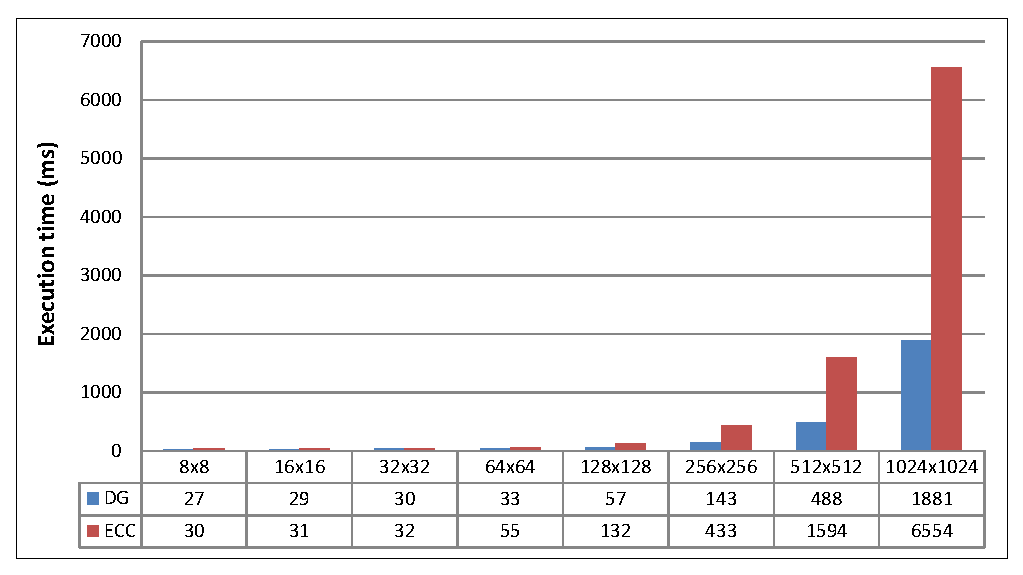
\includegraphics[width=70mm]{./eps/qos_time}
\caption{Execution time under error confinement and ECC}
\vspace{-4mm}
\label{fig:qos_time}
\end{figure}

Proposed approach combined with parity bits achieves much less memory usage than ECC, which is shown in Figure \ref{fig:qos_size}. For small image size under $16 \times 16$, error confinement incurs more spatial overhead than ECC due to its predefined reference matrix of 32-bit floating point words with a size of $8 \times 8$. However, the ECC approach which applies Hamming code scheme $H[38, 32]$ incurs 18.75\% of memory overhead for each protected data word. Consequently, the extra memory used by ECC goes far beyond the ones of proposed approach for larger images. For the image size of $1,024 \times 1,024$, ECC consumes \textbf{5.99}$\times$ the memory used by proposed approach, which closely approximates the theoretical ratio between the 6 bits ECC and 1 bit parity.

\begin{figure}
\centering
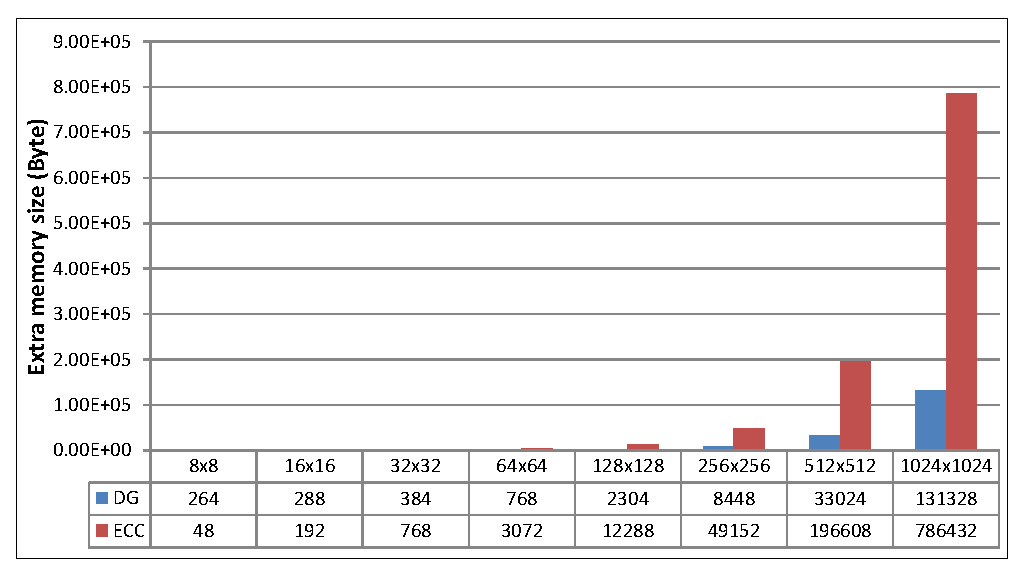
\includegraphics[width=70mm]{./eps/qos_size}
\caption{Size of data memory usage under error confinement and ECC}
\vspace{-4mm}
\label{fig:qos_size}
\end{figure}

\subsection{Architecture Overhead} \label{sec::head_overhead}
The proposed architecture is synthesized at 25MHz under 65nm Faraday technology. Table \ref{tab:qos_overhead} presents the synthesis result compared to the original architecture. It is observed that the architectural extension incurs huge overheads on the original processor in area and power. Further investigation reviews that the logic and registers which record the memory range of protected data, LUT and parity encoding mainly contribute to such overhead. In terms of critical path, the timing cost only has 4.2\% increment since the longest path of the original design, which goes through the hardware multiplier, remains almost unchanged.

\begin{table}[hbt]
\begin{center}
\caption{Overheads for architecture extension}
    \label{tab:qos_overhead}
\begin{tabular}{|c|c|c|c|c|c|}\hline 
                 & \multicolumn{2}{c|}{\textbf{Area}} & \multicolumn{2}{c|}{\textbf{Power}} & \textbf{Critical} \\ 
                 & \multicolumn{2}{c|}{\textbf{(NAND equiv.)}} & \multicolumn{2}{c|}{\textbf{($\mu$Watt)}} & \textbf{path} \\ \cline{2-5}
                 & Comb. & Seq. & Dynamic & Leakage & (ns) \\\hline
Original          & 11789         & 6187       & 206     & 65      & 6.12 \\\hline
QoS extension     & 26519         & 10663      & 349     & 124     & 6.38 \\\hline
Increase (\%)     & 124.9         & 72.3       & 69.4    & 90.8    & 4.2  \\\hline
\end{tabular}
\vspace{-4mm}
\end{center}
\end{table}

\begin{figure}[hbt]
\centering
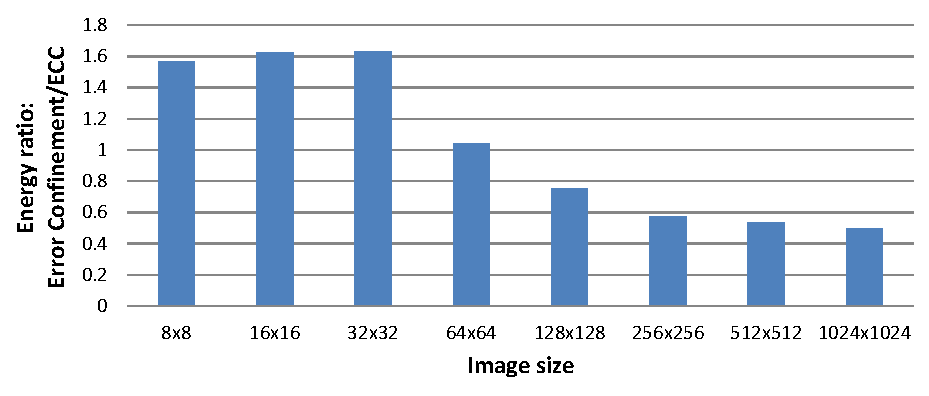
\includegraphics[width=70mm]{./eps/qos_energy}
\caption{Energy ratio between proposed approach and ECC vs image size}
\vspace{-4mm}
\label{fig:qos_energy}
\end{figure}

Although the architecture extension achieves large power overhead, the energy consumption radio between proposed approach and ECC reduces as image size grows, which is illustrated in Figure \ref{fig:qos_energy}. This is because ECC takes longer time to finish. Starting from image size of $128 \times 128$ the proposed approach consumes less energy than ECC, while the energy benefit increases even further for larger images.

